%!TEX program = xelatex
% Note: this template must be compiled with XeLaTeX rather than PDFLaTeX
% due to the custom fonts used. The line above should ensure this happens
% automatically, but if it doesn't, your LaTeX editor should have a simple toggle
% to switch to using XeLaTeX.

\documentclass[
  aspectratio=169, % Uncomment to use an aspect ratio of 16:9 (160 mm by 90 mm)
  %aspectratio=43, % Uncomment to use an aspect ratio of 4:3 (128mm by 96mm)
  t, % Top align all slide content by default
  onlytextwidth, % Typeset content in columns at text width
  10pt, % Default font size, use 10pt for the 16:9 aspect ratio and 8pt for the 4:3 aspect ratio
]{beamer}

\usepackage{../../ImperialTheme/beamer/beamerthemeImperial} % Use the Imperial theme
\usepackage{tikz}
\usetikzlibrary{calc}


\def\imagefolder{../../ImperialTheme/beamer/Images}
\def\Rey{\text{Re}}
\title{Mesh coarsing} % Presentation title to appear on the title slide and left footers

\subtitle{} % Presentation subtitle to appear on the title slide

\author{Víctor Ballester} % Author name(s) to appear on the title slide

\date{\today} % Presentation date to appear on the title slide and right footers

\begin{document}

\begingroup
\setbeamercolor{background canvas}{bg=ICLLightGrey} % Slide background color
\setbeamercolor{title page title}{fg=ICLBlue} % Title text color
\setbeamercolor{title page subtitle}{fg=ICLBlue} % Subtitle text color
\setbeamercolor{author}{fg=ICLBlue} % Author(s) text color
\setbeamercolor{date}{fg=ICLBlue} % Date text color
\setbeamertemplate{title page}[logo]{\imagefolder/ICL_Logo_Blue.pdf} % Imperial logo color, use 'ICL_Logo_White.pdf' for white and 'ICL_Logo_Blue.pdf' for blue
\frame[plain, s]{\titlepage} % Output the title page with no footer ('plain') and vertically distributed text ('s')
\endgroup

\begin{frame}
  \frametitle{Old Mesh vs New mesh (d = 3, w = 26)}
	\begin{itemize}
	  \item Old mesh: $p=5$, 11673 elements.
	  \item New mesh: $p=5$, 2328 elements.
	\end{itemize}


	Most important implementation is that I shortened the dowstream region from $1000\delta^*$ to $500\delta^*$. Initially Jeff told us to use a domain such that at the outflow we have $Re_{\delta^*} = 2000$, but even for the $n$-factor computation I think with half the length we can still have a good approximation of the n-factor curves.

	I mean, for the compressible simulations I was already using $500\delta^*$.
\end{frame}
\begin{frame}
  \frametitle{Mesh comparison (zoomed out)}
  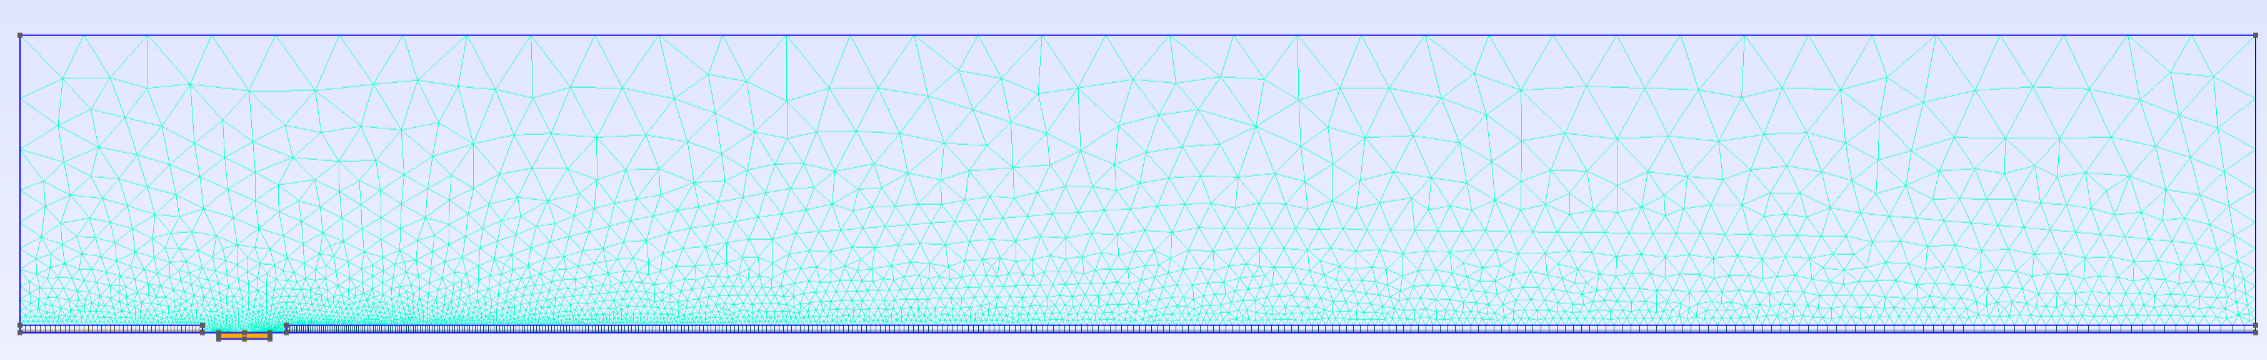
\includegraphics[width=\linewidth]{Images/finemesh.png}
  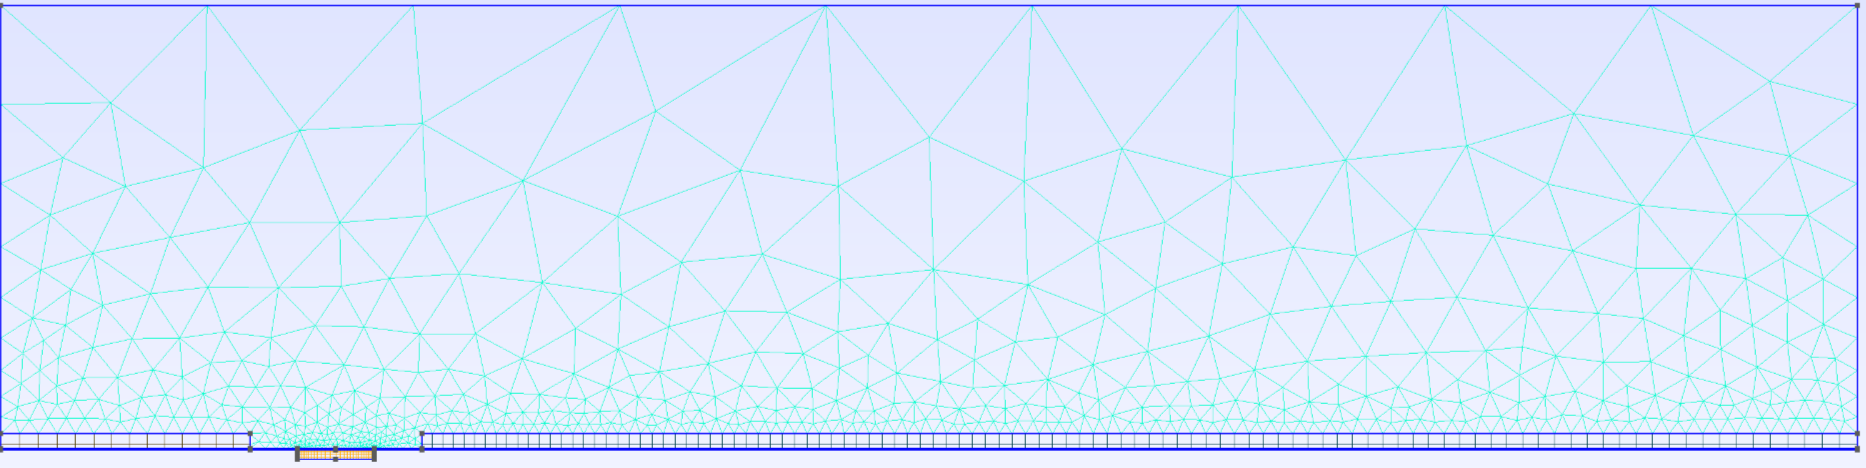
\includegraphics[width=\linewidth]{Images/coarsemesh.png}
\end{frame}
\begin{frame}
  \frametitle{Mesh comparison (zoomed in)}
  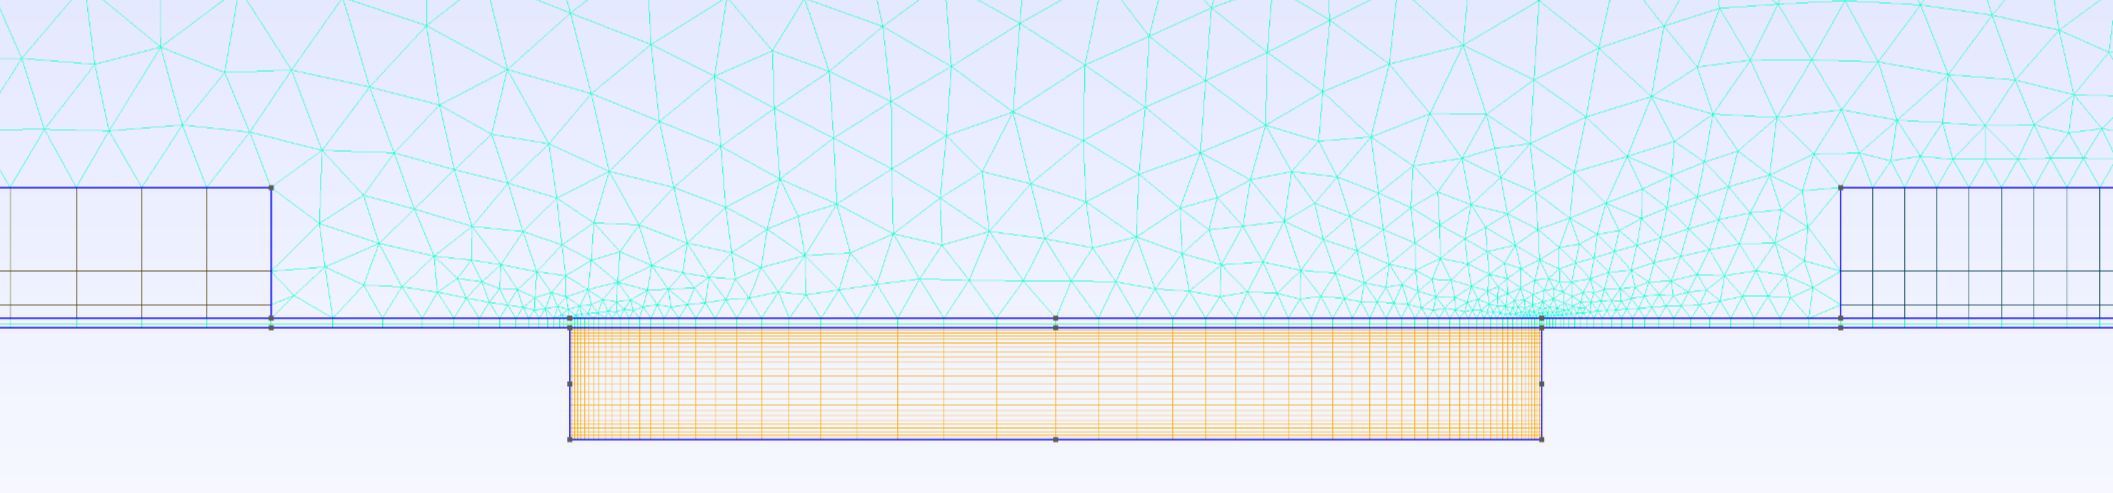
\includegraphics[width=\linewidth]{Images/zoomedfinemesh.png}
  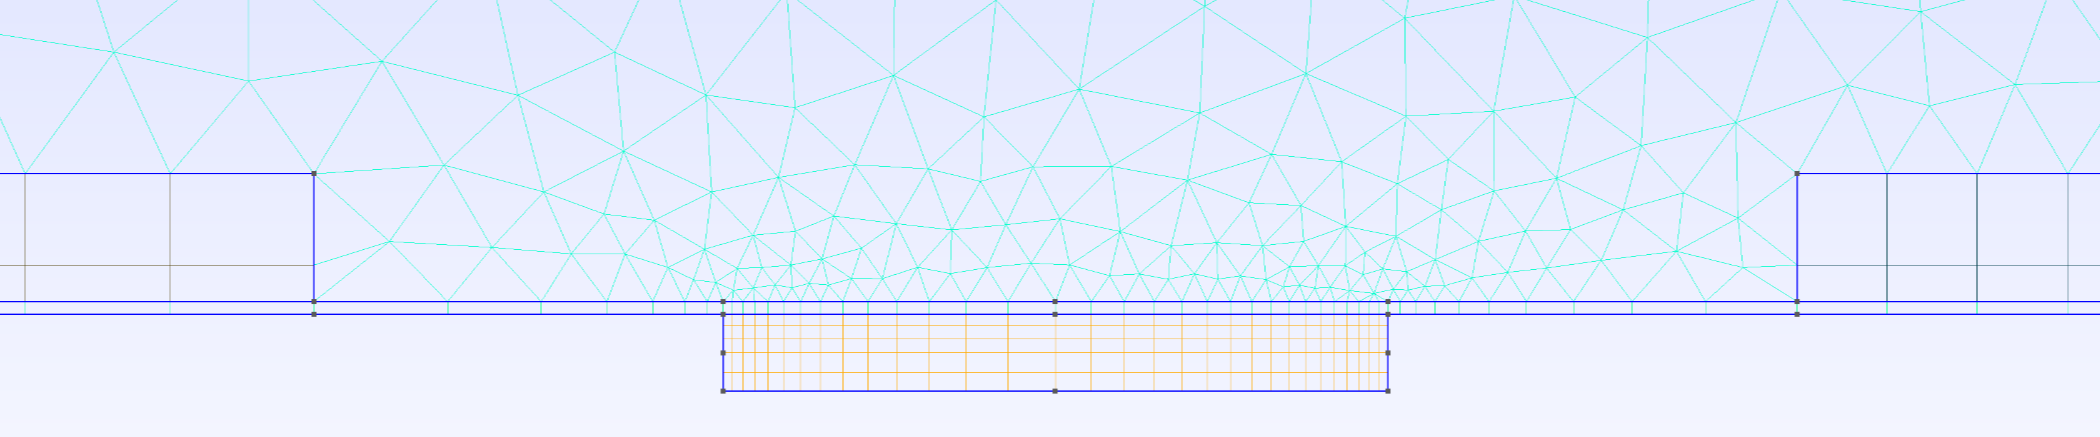
\includegraphics[width=\linewidth]{Images/zoomedcoarsemesh.png}
\end{frame}
\begin{frame}
  \frametitle{Physics comparison}
  \begin{itemize}
    \item L 2 error (variable u): 304.644 (old) vs 304.646 (new)
    \item L inf error (variable u): 1.01793 (old) vs 1.02519 (new)
     \item  L 2 error (variable v): 0.510122 (old) vs 0.590828 (new)
     \item L inf error (variable v): 0.115768 (old) vs 0.157218 (new)
     \item L 2 error (variable p): 0.1737 (old) vs 1.3124 (new)
     \item L inf error (variable p): 0.0527884 (old) vs 0.0949722 (new)
     \item $\omega$: 0.263935 (old) vs 0.264117 (new) 
  \end{itemize}
\end{frame}
\begin{frame}
  \frametitle{Pressure comparison}
  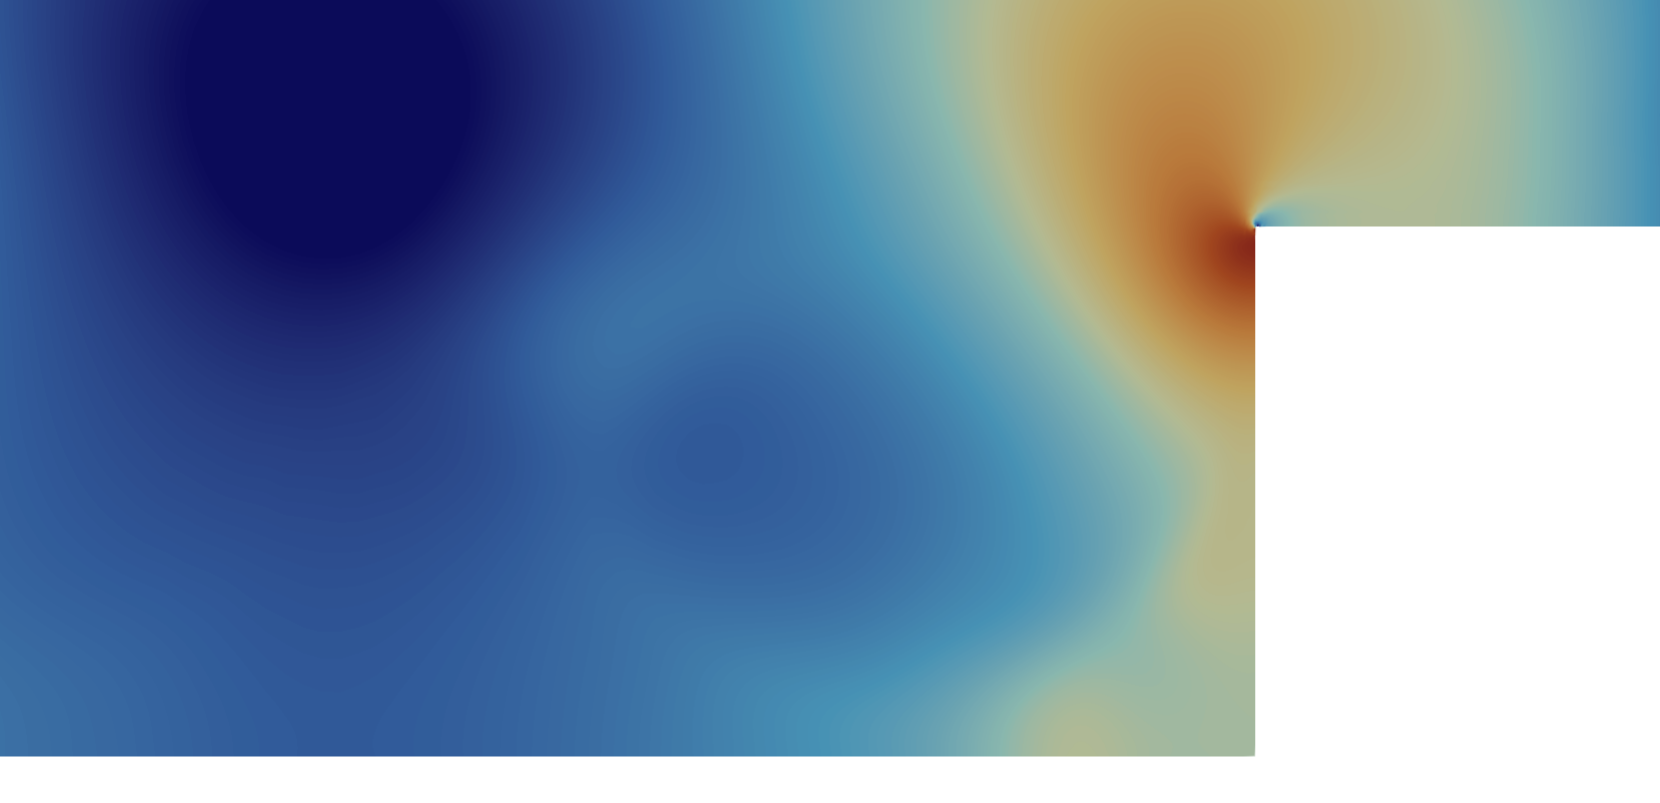
\includegraphics[width=0.5\linewidth]{Images/p_old.png}
  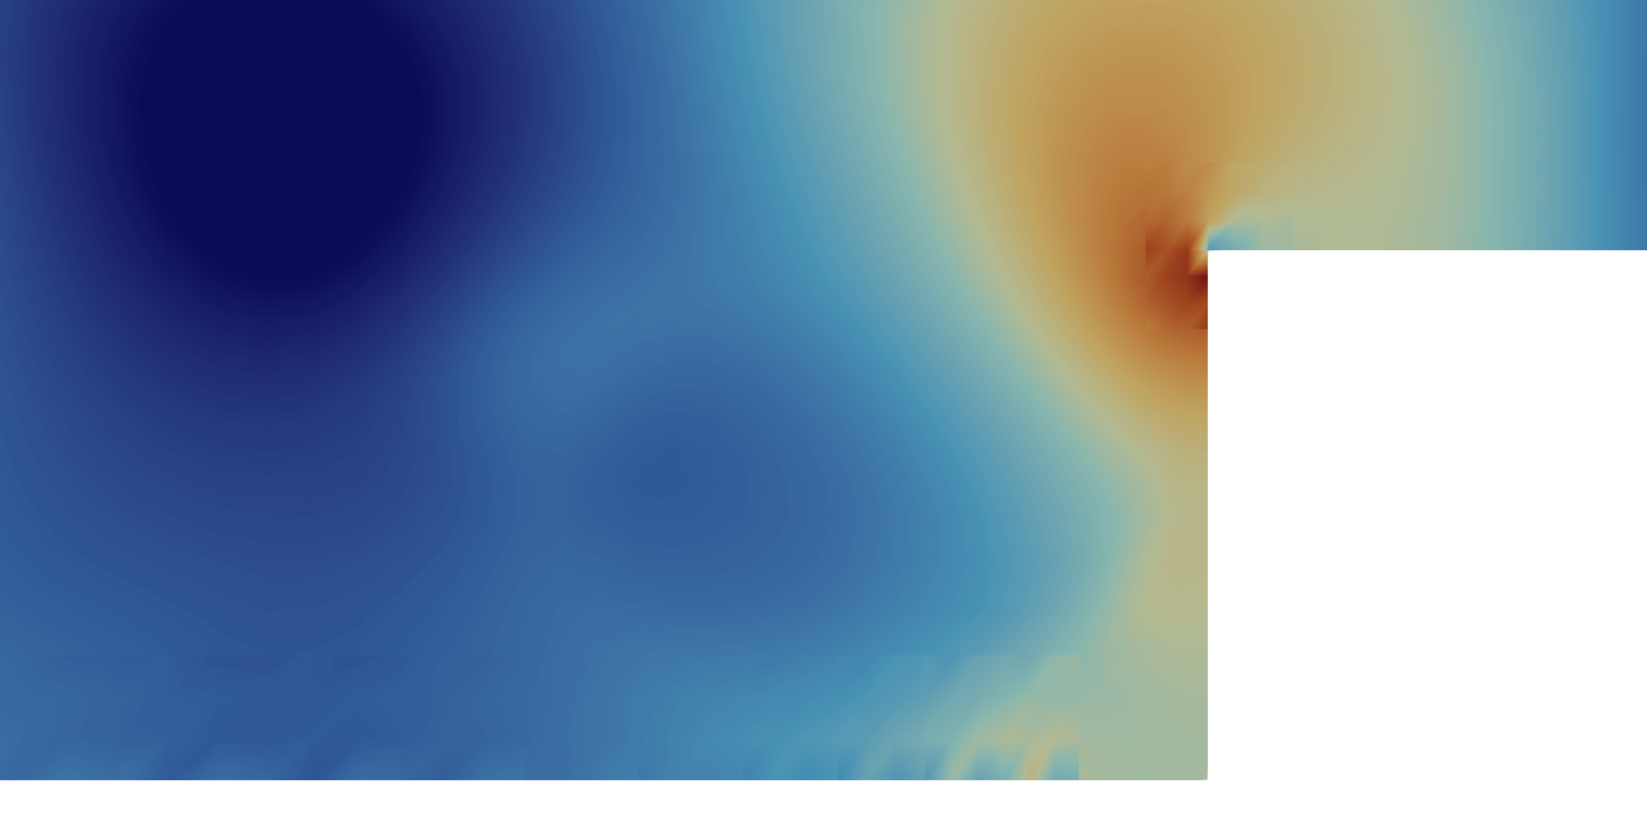
\includegraphics[width=0.5\linewidth]{Images/p_new.png}
\end{frame}
\end{document}
